% \vspace*{-0.2cm}
\section{Experiments}

In this section, we evaluate the performance of our method in both simulation and real-world regimes and conduct ablation studies. 
The demo videos of our method can be found at the \href{https://junfeng-long.github.io/HIMLoco/}{Project Page}.
Additional descriptions of the experimental setup, baselines, and hyper-parameters can be found in the Appendix.

\subsection{Evaluation Setups}

\paragraph{Compared Methods.} We compare our method with the following methods: \\
$\bullet$ Baseline: Train without HIM but keep the source encoder and optimize it with PPO. \\
$\bullet$ Ours w/o velocity input: Set the velocity inputs to the policy network as 0. \\
$\bullet$ Ours w/o velocity loss: Direct remove the velocity estimation. \\
$\bullet$ Ours w/o internal latent input: Set the internal latent inputs to the policy network as 0. \\
$\bullet$ Ours w/o internal latent loss: Direct remove the internal latent estimation. \\
$\bullet$ Regression: Optimize the hybrid internal model with regression methods. \\
$\bullet$ Oracle: Train the policy with a history of full observations. \\
$\bullet$ Rapid Motor Adaptation~\citep{kumar2021rma}. \\
$\bullet$ Multiplicity of Behavior (Walk These Ways)~\citep{margolis2023walk}. \\
$\bullet$ Onboard MPC controller, which is only compared in real-world experiments. 

\paragraph{Setups in the Real World.}
\label{exp:real}
We deploy our policy on Unitree A1, Go1, and Aliengo. The policy runs at 50 Hz, with a PD controller running at 500 Hz to track the target.
The parameters are $k_p = 30.0$, $k_d = 0.75$ for A1 and Go1, $k_p = 40.0$, $k_d = 2.0$ for Aliengo. 
We compare methods with robust tests in the real world, with 3 benchmarks and 8 tasks.
The details can be found in Appendix~\ref{app:real}.

\paragraph{Setups in Simulations.} 
In simulations, we compare methods according to the tracking errors. 
The tracking errors for linear velocity and angular velocity are quantified using the norms $\|v_{x,y} - v_{x,y}^{\text{target}}\|_2$ and $\|\omega_{\text{yaw}} - \omega_{\text{yaw}}^{\text{target}}\|_2$, respectively. 
We test the tracking performance under various terrain conditions and motion ranges. 
A detailed description can be found in Appendix~\ref{app:simu}.

\subsection{Main Results}
\begin{table}[t]
\vspace{-1cm}
\centering
\caption{Main results with average performance~$\uparrow$ in the real-world benchmarks over 20 trials, where $\pm$ captures a $95\%$ confidence interval. The top results are highlighted.
}
\resizebox{\linewidth}{!}{%
\begin{tabular}{ccccccc}
\toprule[1.5pt]
Benchmarks &
  Environments &
  Metrics &
  \textbf{Ours} &
  RMA &
  MoB &
  Built-in MPC \\ \midrule[1.5pt]
\multirow{2}{*}{Stairs} &
  \begin{tabular}[c]{@{}c@{}}Short-range \\(A1)\end{tabular} &
  \begin{tabular}[c]{@{}c@{}}Success rate \\(\%)\end{tabular} &
  \hl{100} &
  60 &
  0 &
  0 \\ \cmidrule{2-7}
 &
  \begin{tabular}[c]{@{}c@{}}Long-range \\(Aliengo)\end{tabular} &
  \begin{tabular}[c]{@{}c@{}}Number of stairs\end{tabular} &
  \hl{176.5±7.81} &
  75.35±19.98 &
  0.0±0.0 &
  0.0±0.0 \\ \midrule
\multirow{2}{*}{\begin{tabular}[c]{@{}c@{}}Unseen \\ Terrains\end{tabular}} &
  \begin{tabular}[c]{@{}c@{}}Compositional \\ Terrain (Aliengo)\end{tabular} &
  \begin{tabular}[c]{@{}c@{}}Success rate \\(\%)\end{tabular} &
  \hl{85} &
  45 &
  0 &
  0 \\ \cmidrule{2-7} 
 &
  \begin{tabular}[c]{@{}c@{}}Deformable\\Slope (A1)\end{tabular} &
  \begin{tabular}[c]{@{}c@{}}Success rate \\(\%)\end{tabular} &
  \hl{55} &
  10 &
  0 &
  0 \\ \midrule
\multirow{4}{*}{\begin{tabular}[c]{@{}c@{}}Anti-\\ disturbance\end{tabular}} &
  \begin{tabular}[c]{@{}c@{}}Dragging\\Obstacle (A1)\end{tabular} &
  \begin{tabular}[c]{@{}c@{}}Maximum weight \\(Kg)\end{tabular} &
  \hl{10} &
  \hl{10} &
  7 &
  3 \\ \cmidrule{2-7} 
 &
  \begin{tabular}[c]{@{}c@{}}Vertical Hit \\(A1)\end{tabular} &
  \begin{tabular}[c]{@{}c@{}}Maximum weight \\(Kg)\end{tabular} &
  \hl{8} &
  \hl{7.5} &
  7 &
  5 \\ \cmidrule{2-7} 
 &
  \begin{tabular}[c]{@{}c@{}}Payload \\(A1)\end{tabular} &
  \begin{tabular}[c]{@{}c@{}}Maximum weight \\(Kg)\end{tabular} &
  \hl{8} &
  7 &
  4 &
  7 \\ \cmidrule{2-7} 
 &
  \begin{tabular}[c]{@{}c@{}}Missing steps \\(Aliengo)\end{tabular} &
  \begin{tabular}[c]{@{}c@{}}Success rate \\(\%)\end{tabular} &
  \hl{100} &
  0 &
  0 &
  0 \\ 
\bottomrule[1.5pt]
\end{tabular}
%
}
\label{real_comp_table}
\end{table}

\paragraph{Real-world Results}
In our real-world benchmarks, we compare our method with RMA~\citep{kumar2021rma}, MoB~\citep{margolis2023walk}, and Built-in MPC. 
The results in Table~\ref{real_comp_table} show our method outperforms the other methods on all tasks and maintains more natural gaits.
It proves that our method can well inherit the policy in simulation and can be deployed to the real world easily.
We also observe that our method can perform very well with high-difficulty tasks such as long-range stairs and the cases never occurred in the training process such as compositional terrains, and deformable slopes, revealing an excellent generalizability in the open world. 


\paragraph{Simulation Results}
In our simulation benchmarks, we compare our method with Baseline, Regression, RMA~\citep{kumar2021rma} and MoB~\citep{margolis2023walk} with Unitree Aliengo.
Results in Table~\ref{sim_tracking_table} show that our method outperforms the other methods on almost all tasks. 
Our method holds more performance improvements than the other methods and significantly outperforms the Regression method. 
Besides, our method also performs better in 66.67\% of the velocity range on easy terrain.


\begin{table}[t]
\vspace{-1cm}
\centering
\caption{Average tracking error~$\downarrow$ in simulation over $4096 \times 5$ trials. Top results are highlighted.
}
\resizebox{\linewidth}{!}{%
\begin{tabular}{@{}cclccccc@{}}
\toprule[1.5pt]
Terrain Types &
  Velocity Types &
  \multicolumn{1}{c}{Ranges} &
  \textbf{Ours} &
  Regression &
  RMA &
  Baseline &
  MoB (Trot) \\ \midrule[1.5pt]
\multirow{8}{*}{Slopes} &
  \multirow{2}{*}{Linear} &
  {[}-1, 1{]} m/s &
  0.073 &
  \hl{0.071} &
  0.158 &
  0.271 &
  0.103 \\ \cmidrule(l){3-8} 
                        &                           & {[}-2, 2{]} m/s   & \hl{0.075} & 0.077 & 0.270 & 0.305 & 0.126 \\ \cmidrule(l){2-8} 
                        & \multirow{2}{*}{Angular}  & {[}-1, 1{]} rad/s & 0.084 & 0.086 & 0.091 & 0.164 & \hl{0.081} \\ \cmidrule(l){3-8} 
                        &                           & {[}-2, 2{]} rad/s & 0.124 & 0.130 & 0.134 & 0.202 & \hl{0.114} \\ \cmidrule(l){2-8} 
                        & \multirow{4}{*}{Combined} & {[}-1, 1{]} m/s   & 0.078 & 0.075 & 0.155 & 0.207 & \hl{0.069} \\ %\cmidrule(l){3-8} 
                        &                           & {[}-1, 1{]} rad/s & \hl{0.047} & 0.050 & 0.074 & 0.143 & 0.052 \\ \cmidrule(l){3-8} 
                        &                           & {[}-2, 2{]} m/s   & \hl{0.094} & 0.107 & 0.203 & 0.224 & 0.103 \\ %\cmidrule(l){3-8} 
                        &                           & {[}-2, 2{]} rad/s & \hl{0.067} & 0.071 & 0.102 & 0.157 & 0.069 \\ \midrule
\multirow{8}{*}{\begin{tabular}[c]{@{}c@{}}Rough\\ Slopes\end{tabular}} &
  \multirow{2}{*}{Linear} &
  {[}-1, 1{]} m/s &
  \hl{0.086} &
  0.091 &
  0.201 &
  0.287 &
  0.105 \\ \cmidrule(l){3-8} 
                        &                           & {[}-2, 2{]} m/s   & \hl{0.085} & 0.088 & 0.294 & 0.331 & 0.124 \\ \cmidrule(l){2-8} 
                        & \multirow{2}{*}{Angular}  & {[}-1, 1{]} rad/s & \hl{0.097} & 0.108 & 0.142 & 0.160 & 0.119 \\ \cmidrule(l){3-8} 
                        &                           & {[}-2, 2{]} rad/s & 0.143 & 0.150 & 0.147 & 0.187 & \hl{0.135} \\ \cmidrule(l){2-8} 
                        & \multirow{4}{*}{Combined} & {[}-1, 1{]} m/s   & \hl{0.088} & 0.095 & 0.167 & 0.220 & 0.147 \\ %\cmidrule(l){3-8}
                        &                           & {[}-1, 1{]} rad/s & \hl{0.054} & 0.070 & 0.086 & 0.169 & 0.092 \\ \cmidrule(l){3-8}
                        &                           & {[}-2, 2{]} m/s   & \hl{0.103} & 0.137 & 0.221 & 0.284 & 0.195 \\ %\cmidrule(l){3-8} 
                        &                           & {[}-2, 2{]} rad/s & \hl{0.076} & 0.096 & 0.117 & 0.201 & 0.114 \\ \midrule
\multirow{4}{*}{Stairs} & Linear                    & {[}-1, 1{]} m/s   & \hl{0.147} & 0.194 & 0.306 & 0.377 & 1.108 \\ \cmidrule(l){2-8} 
                        & Angular                   & {[}-1, 1{]} rad/s & \hl{0.087} & 0.101 & 0.241 & 0.370 & 0.930 \\ \cmidrule(l){2-8} 
                        & \multirow{2}{*}{Combined} & {[}-1, 1{]} m/s   & \hl{0.135} & 0.217 & 0.337 & 0.405 & 1.270 \\ %\cmidrule(l){3-8} 
                        &                           & {[}-1, 1{]} rad/s & \hl{0.096} & 0.154 & 0.201 & 0.289 & 0.992 \\ \midrule
\multirow{4}{*}{\begin{tabular}[c]{@{}c@{}}Discretre\\ Obstacles\end{tabular}} &
  Linear &
  {[}-1, 1{]} m/s &
  \hl{0.125} &
  0.182 &
  0.311 &
  0.279 &
  0.973 \\ \cmidrule(l){2-8} 
                        & Angular                   & {[}-1, 1{]} rad/s & \hl{0.083} & 0.097 & 0.175 & 0.253 & 0.841 \\ \cmidrule(l){2-8} 
                        & \multirow{2}{*}{Combined} & {[}-1, 1{]} m/s   & \hl{0.125} & 0.206 & 0.305 & 0.374 & 1.254 \\ %\cmidrule(l){3-8} 
                        &                           & {[}-1, 1{]} rad/s & \hl{0.075} & 0.133 & 0.177 & 0.246 & 0.976 \\ 
                        \bottomrule[1.5pt]
\end{tabular}
%
}
\label{sim_tracking_table}
\end{table}


\subsection{Ablation Studies}
\label{ablation}
\paragraph{Ablation Studies in Simulations.}
We mainly conduct ablation studies in simulation with Aliengo. The metrics include the normalized linear velocity tracking score, the normalized angular velocity tracking score, and the maximum reachable terrain level.
The task and command sampling are described in Section~\ref{curriculum}. The definition of terrain levels can be found in Appendix~\ref{app:terrain}. Terrains include rough flats, pyramid slopes, rough pyramid slopes, wave terrain, stairs, and flats with discrete obstacles, and the corresponding proportion is [0.1, 0.2, 0.6, 0.1]. The normalized linear velocity tracking score (NLTS) and the normalized angular velocity tracking score (NATS) are:
\begin{align*}
        \text{NLTS } = \text{exp}(-\frac{\|v_{x,y} - v_{x,y}^{\text{target}}\|^2_2}{0.25}), \text{  }
        \text{NATS } = \text{exp}(-\frac{\|\omega_{\text{yaw}} - \omega_{\text{yaw}}^{\text{target}}\|^2_2}{0.25}).
\end{align*}
The results are shown in Fig.~\ref{ablation_figure}, in which the curves are averaged over 10 seeds. 
The shaded area represents the standard deviation across seeds. 
Despite our method does not need terrain information, it exhibits the most similar results to the Oracle policy.
We also conclude that:

1. In our hybrid internal model, both internal embedding and velocity estimation improve the policy. The absence of any of them can lead to performance degradation.\\
2. Our hybrid internal optimization outperforms the Regression method. It proves that our method can utilize batch-level information to better understand the properties of different terrains. \\
3. RMA can not imitate all the great performances of Oracle. Our method maintains consistent observations between simulation and reality and results in better performance. 

\paragraph{Ablation Studies in the Real World.}
We also conduct ablation studies on our real-world benchmarks. Results in Table~\ref{real_ablation_table} show that our hybrid internal model contributes to the performance, with the internal model playing a critical role.

\begin{figure}[t]
    \label{ablation_figure}
    \centering
    % \vspace*{-0.3cm}
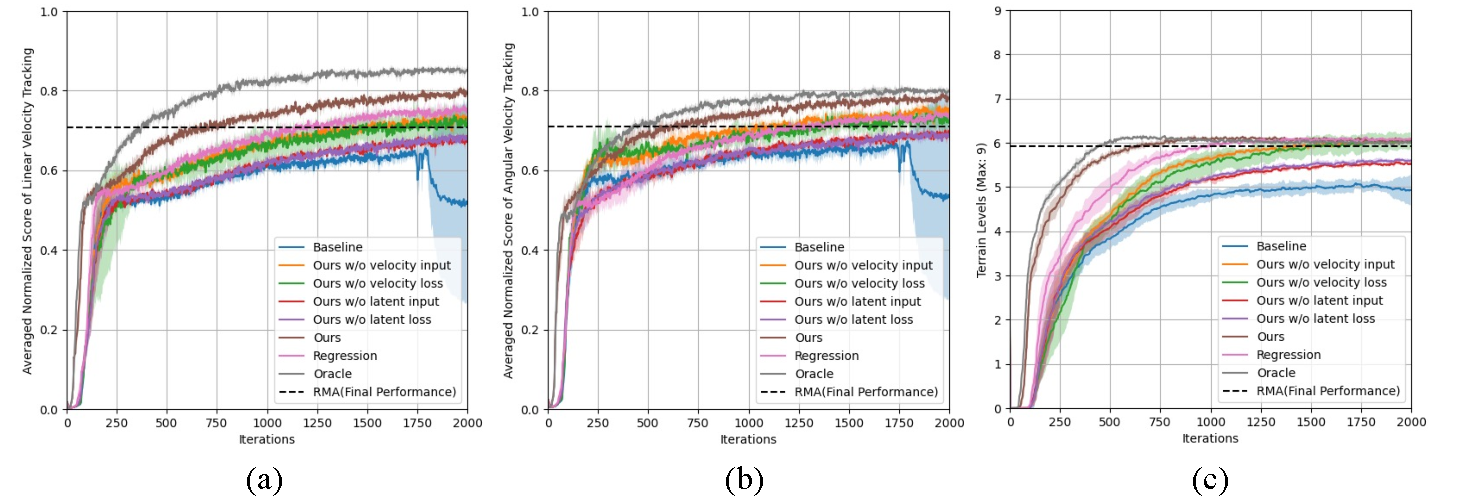
\includegraphics[width=1.0\textwidth]{plot_curve.pdf}
    \label{fig:lin_curve}
    % \vspace*{-0.4cm}
    \caption{Ablation studies with learning curves of (a) normalized linear velocity tracking score, (b) normalized angular velocity tracking score, and (c) maximum reachable terrain level in Isaac Gym.}
    % \vspace*{-0.3cm}
\end{figure}

\begin{table}[t]
% \vspace*{-0.8cm}
\centering
\caption{Ablation studies with average performance~$\uparrow$ in the real-world benchmarks over 20 trials, where $\pm$ captures a $95\%$ confidence interval. Top performances are highlighted.}
\resizebox{\linewidth}{!}{%
\begin{tabular}{cccccccccc}
\toprule[1.5pt]
Benchmarks &
  Environments &
  Metrics &
  \textbf{Ours} &
  \begin{tabular}[c]{@{}c@{}}Ours w/o \\ vel. inp.\end{tabular} &
  \begin{tabular}[c]{@{}c@{}}Ours w/o \\ vel. loss\end{tabular} &
  \begin{tabular}[c]{@{}c@{}}Ours w/o \\ lat. inp.\end{tabular} &
  \begin{tabular}[c]{@{}c@{}}Ours w/o \\ lat. loss\end{tabular} &
  Regression &
  Baseline \\ \midrule[1.5pt]
\multirow{2}{*}{Stairs} &
  \begin{tabular}[c]{@{}c@{}}Short-range\\ (A1)\end{tabular} &
  \begin{tabular}[c]{@{}c@{}}Success \\rate (\%)\end{tabular} &
  \hl{100} &
  85 &
  80 &
  50 &
  55 &
  85 &
  10 \\ \cmidrule{2-10} 
 &
  \begin{tabular}[c]{@{}c@{}}Long-range\\ (Aliengo)\end{tabular} &
  \begin{tabular}[c]{@{}c@{}}Number \\ of stairs\end{tabular} &
  \hl{176.5±7.81} &
  51.45±25.67 &
  54.6±24.68 &
  13.3±13.42 &
  10.6±9.68 &
  155.7±13.48 &
  0.0±0.0 \\ \midrule
\multirow{2}{*}{\begin{tabular}[c]{@{}c@{}}Unseen \\ Terrains\end{tabular}} &
  \begin{tabular}[c]{@{}c@{}}Compositional \\ Terrain (Aliengo)\end{tabular} &
  \begin{tabular}[c]{@{}c@{}}Success \\rate (\%)\end{tabular} &
  \hl{85} &
  70 &
  75 &
  50 &
  50 &
  70 &
  15 \\ \cmidrule{2-10} 
 &
  \begin{tabular}[c]{@{}c@{}}Deformable \\Slope (A1)\end{tabular} &
  \begin{tabular}[c]{@{}c@{}}Success \\rate (\%)\end{tabular} &
  \hl{55} &
  30 &
  25 &
  0 &
  0 &
  30 &
  0 \\ \midrule
\multirow{4}{*}{\begin{tabular}[c]{@{}c@{}}Anti-\\ disturbance\end{tabular}} &
  \begin{tabular}[c]{@{}c@{}}Dragging \\Obstacle (A1)\end{tabular} &
  \begin{tabular}[c]{@{}c@{}}Maximum \\ weight (Kg)\end{tabular} &
  \hl{10} &
  \hl{10} &
  \hl{10} &
  5 &
  5 &
  \hl{10} &
  4 \\ \cmidrule{2-10} 
 &
  \begin{tabular}[c]{@{}c@{}}Vertical Hit\\ (A1)\end{tabular} &
  \begin{tabular}[c]{@{}c@{}}Maximum \\ weight (Kg)\end{tabular} &
  \hl{8} &
  7 &
  6.5 &
  4 &
  4 &
  8 &
  5.5 \\ \cmidrule{2-10} 
 &
  \begin{tabular}[c]{@{}c@{}}Payload\\ (A1)\end{tabular} &
  \begin{tabular}[c]{@{}c@{}}Maximum \\ weight (Kg)\end{tabular} &
  \hl{8} &
  7 &
  7 &
  3.5 &
  3.5 &
  \hl{7.5} &
  3 \\ \cmidrule{2-10} 
 &
  \begin{tabular}[c]{@{}c@{}}Missing steps\\ (Aliengo)\end{tabular} &
  \begin{tabular}[c]{@{}c@{}}Success \\rate (\%)\end{tabular} &
  \hl{100} &
  90 &
  90 &
  5 &
  0 &
  65 &
  0 \\ \bottomrule[1.5pt]
\end{tabular}
%
}
\label{real_ablation_table}
% \vspace*{-0.4cm}
\end{table}


